\documentclass[]{mangos-musings}
\usepackage[dvipsnames]{xcolor}
\allowdisplaybreaks
\usepackage{array}
\usepackage{multicol}
\pagenumbering{gobble}
\begin{document}
\title{21-259 Recitations \hfill \small{tylery}}
\tableofcontents

\newpage
\section{08-26-2025}
\subsection{Basics}
This class is \textbf{Calculus in Three Dimensions}, thus the class will require you to think in 3-D.
\begin{itemize}
  \item Get used to drawing in 3-D. 
  \\ My preference is to draw the usual vertical and horizontal axes. 
  \\ Label the horizontal axis $y$ and the vertical axis $z$. 
  \\ Then draw a diagonal from the bottom left to the top right, passing through the origin. Label this axis $x$.
  Note that you can interchange any of the axis labels as necessary (which will come in handy when we start doing 3-D integration). 
  \item In $\R^3$, the (Euclidean) distance (also referred to as the $L_2$ norm) between any two points $(x_1, y_1, z_1)$ and $(x_2, y_2, z_2)$
  is given by the formula 
  \[d = \sqrt{(x_2 - x_1)^2 + (y_2 - y_1)^2 + (z_2 - z_1)^2}\]
\end{itemize}
\subsection{Planes and Spheres}
In this course, you will often deal with planes and spheres (e.g., spherical coordinates). 
\begin{itemize}
  \item You will learn the canonical formula for a plane later (finding it involves cross products). For now, we will find equations for planes parallel to another plane.
  \item[Ex.] Write an equation of the plane passing through point $(21, 2, 59)$ that is parallel to the $xz$-plane.
  \subitem When a plane is parallel to the $xz$-plane, it means only the $x$ and $z$ coordinates may vary. 
  \subitem Thus taking the $y$-value, we get the equation $y = 2$.
  \item[Ex.] Write an equation of the plane passing through points $(2, 125, 9), (21, 25, 9), (5, 7, 9)$ that is parallel to the $xy$-plane. 
  \subitem When a plane is parallel to the xy-plane, it means only the x and y coordinates may vary. 
  \subitem Conveniently, the $z$-value in all 3 coordinates are equal; we get the equation $z = 9$.
  \item A sphere is the set of all points in space equidistant from a fixed point, the center of
  the sphere. For center $(a, b, c)$ and radius $r$, we represent the sphere by the (``canonical'') equation: 
  \[(x-a)^2 + (y-b)^2 + (z-c)^2 = r^2\]
  \item[Ex.] Find the equation of the sphere with diameter $\overline{PQ}$ where $P = (2, -1, -3)$ and $Q = (-2, 5, -1)$.
  \subitem First, find the center, which is at the midpoint of the diameter $\overline{PQ}$:
  \[C = \left(\dfrac{2 + (-2)}{2}, \dfrac{-1 + 5}{2}, \dfrac{-3 + (-1)}{2}\right) = \left(0, 2, -2\right)\]
  \subitem Next, find the radius using the distance formula (half the length of the diameter)
  \[r = \dfrac{1}{2}\norm{\overline{PQ}} 
      = \dfrac{1}{2}\sqrt{(-2 - 2)^2 + (5 - (-1))^2 + (-1 - (-3))^2}
      = \dfrac{1}{2}\sqrt{56}
      = \sqrt{\dfrac{56}{4}}
      = \sqrt{14}\]
  \subitem Thus the sphere is given by $x^2 + (y-2)^2 + (z+2)^2 = 14$
\end{itemize}
\subsection{Vector Notation}
Vectors are quantities with magnitude and direction. In $\R^3$, the standard unit vectors are 
\[\hat{i} = \langle1, 0, 0\rangle \quad \hat{j} = \langle0, 1, 0\rangle \quad \hat{k} = \langle0, 0, 1\rangle \]

There are several notations. Fix points in $\R^3$ $P = (0, 2, 1)$ and $Q = (2, 5, 9)$
\\ Let's represent the vector $\overrightarrow{PQ} = \langle x_Q - x_P, y_Q - y_P, z_Q - z_P\rangle$.
\begin{itemize}
  \item Component Form: $\overrightarrow{PQ} = \langle 2-0, 5-2, 9-1\rangle = \langle 2, 3, 8\rangle$
  \item Using the unit vectors: $\overrightarrow{PQ} = 2\hat{i} + 3\hat{j} + 8\hat{k}$
\end{itemize}

Ex: Consider the vectors $v = \langle 0, 2, 1\rangle$ and $u = \langle 2, 5, 9\rangle$. Find a unit vector in the direction of $3v + u$. 

You will need the following rules (taken from your textbook)
\\ 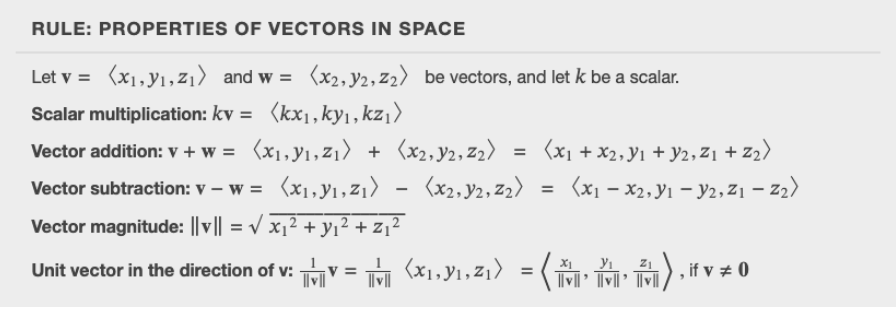
\includegraphics{assets/rec01-vectorspace.png}

Solution: first find $3v + u$, then find unit vector in that direction.
\begin{align*}
  3v + u &= \langle 3(0), 3(2), 3(1)\rangle + \langle 2, 5, 9\rangle \tag{scalar multiplication}
  \\ &=  \langle 0, 6, 3\rangle +  \langle 2, 5, 9\rangle 
  = \langle 2, 11, 12\rangle
  \\ \dfrac{1}{\norm{3v + u}} (3v + u) &= \dfrac{\langle 2, 11, 12\rangle}{\sqrt{2^2 + 11^2 + 12^2}} =  \langle \dfrac{2}{\sqrt{269}}, \dfrac{11}{\sqrt{269}}, \dfrac{12}{269}\rangle \tag{unit vector in direction}
\end{align*}
Observe that $269$ is prime, so you can't simplify the denominator. Thus we're done. Not all numbers will be pretty, but as a tip: make sure your answers are feasible. If you are taking the length of a vector with 1-digit coordinates and get a 5-digit number, that's probably wrong. 
\\ \textbf{DON'T FORGET THE SQUARE ROOT $\sqrt{}$ when taking norms!!!!}

\newpage
\subsection{Computing 3x3 Determinants}
Useful for computing cross products. You are free to use whatever trick you want so long as you show your work. (note vertical bars means determinant, while square brackets mean matrix). 

\subsubsection{Cofactor Method}
Key notes: $+, -, +$ (\textbf{DON'T FORGET THE MIDDLE IS NEGATIVE}) and the 2x2 sub-determinants are the elements not in the same row or column.
\begin{align*}
  \begin{vmatrix}
    a & b & c \\
    d & e & f \\ 
    g & h & i
  \end{vmatrix}
  &= a \begin{vmatrix}
    e & f \\ 
    h & i
  \end{vmatrix}
  - b \begin{vmatrix}
    d & f \\ 
    g & i
  \end{vmatrix}
  + c \begin{vmatrix}
    d & e \\ 
    g & h
  \end{vmatrix}
  = a(ei - fh) - b(di - fg) + c(dh - eg)
  \\ &= aei - afg - bdi + bfg + cdh - ceg
\end{align*}
For cross products between two vectors $u = \langle u_x, u_y, u_z \rangle$ and $v = \langle v_x, v_y, v_z \rangle$, you just compute the 3x3 determinant $\begin{vmatrix}
  \hat{i} & \hat{j} & \hat{k} \\ 
  u_x & u_y & u_z \\ 
  v_x & v_y & v_z
\end{vmatrix}$

\subsubsection{Diagonal Method}
Recall that the 2x2 determinant is computed using the diagonals:
$\begin{vmatrix}
    a & b \\
    c & d 
\end{vmatrix} = ad - bc$, where the diagonals going from right to left are positive and diagonals going from left to right are negative. We extend this idea to 3x3 determinants:
\[\begin{vmatrix}
    a & b & c \\
    d & e & f \\ 
    g & h & i
  \end{vmatrix} \xRightarrow{expand} \begin{matrix}
    & & a & b & c & & \\
    & f & d & e & f & d & \\ 
    h & i & g & h & i & g & h
  \end{matrix} \xRightarrow{compute} aei + bfg + cdh - afh - bdi - ceg\]
which is the same result as derived from the cofactor method.


\newpage
\section{08-28-2025}
\subsection{Section 2.3, Checkpoint 2.23: Finding the Angle between Two Vectors}
Find the measure of the angle, in radians, formed by vectors $a=\langle1,2,0\rangle$ and $b=\langle2,4,1\rangle$. Round to the nearest hundredth.
\begin{align*}
  \\ 
  \\ 
  \\ 
  \\
\end{align*}

\subsection{Section 2.3, Checkpoint 2.24: Identifying Orthogonal Vectors}
For which value of $x$ is $p=\langle2,8,-1\rangle$ orthogonal to $q=\langle x,-1,2\rangle$?
\begin{align*}
  \\ 
  \\ 
  \\
\end{align*}

\subsection{Section 2.3, Checkpoint 2.27: Resolving Vectors into Components}
Express $v=5i-j$ as a sum of orthogonal vectors such that one of the vectors has the same direction as $u=4i+2j$.
\begin{align*}
  \\ 
  \\
  \\
  \\
\end{align*}
\begin{center}
  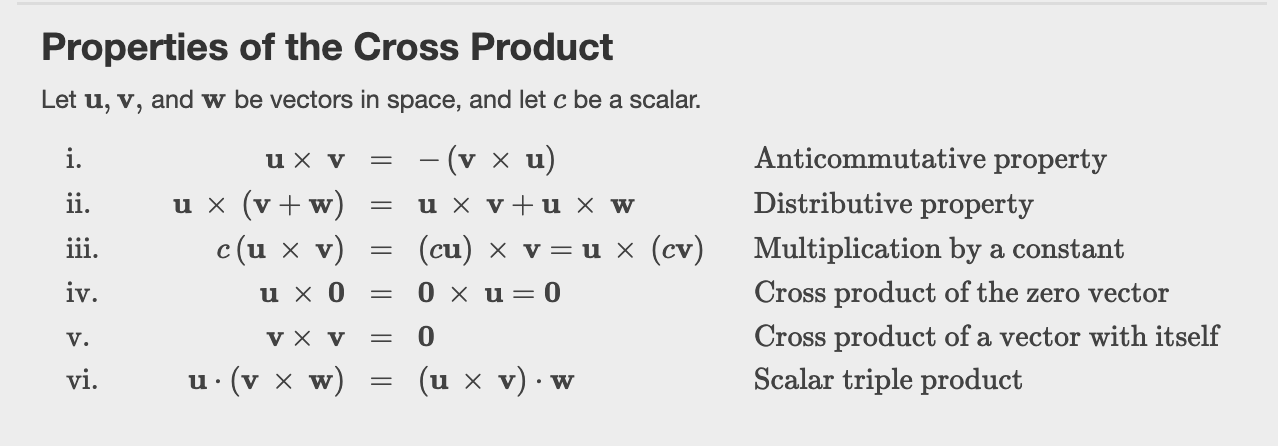
\includegraphics[scale=0.6]{assets/rec02-crossprod-properties.png}
\end{center}
\subsection{Section 2.4, Checkpoint 2.33 (quick)}
Use the properties of the cross product to calculate $(i\times k)\times(k\times j)$.
\begin{align*}
  \\ 
  \\ 
  \\ 
  \\
\end{align*}
\subsection{Section 2.4, Checkpoint 2.38}
Find the area of the parallelogram $PQRS$ with vertices $P(1,1,0),Q(7,1,0),R(9,4,2)$, and $S(3,4,2)$.
\begin{align*}
  \\ 
  \\ 
  \\ 
  \\
  \\
  \\
\end{align*}

\subsection{Section 2.4, Example 2.44: Evaluating Torque}
A bolt is tightened by applying a force of 6 N to a 0.15-m wrench (Figure 2.62). The angle between the wrench and the force vector is 40°. Find the magnitude of the torque about the center of the bolt. Round the answer to two decimal places.

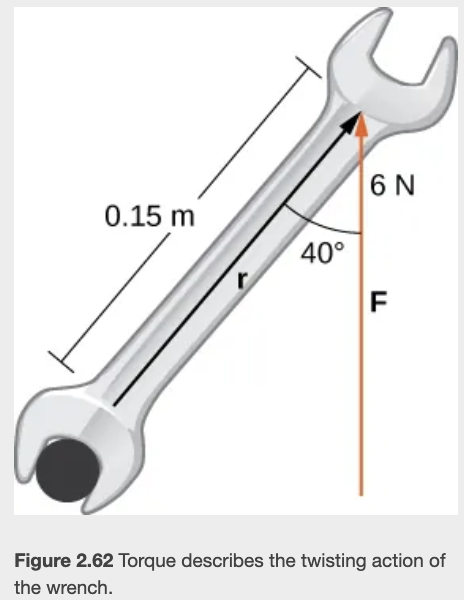
\includegraphics[scale=0.8]{assets/rec02-fig-2.62.png}




\newpage
\section{09-02-2025}
\subsection{Section 2.5, Checkpoint 2.45}
Find the distance between point $(0,3,6)$ and the line with parametric equations 
\[x=1-t,y=1+2t,z=5+3t\]
\begin{align*}
  \\ 
  \\ 
  \\ 
  \\
  \\
  \\
  \\
  \\
  \\
  \\
\end{align*}


\subsection{Section 2.5, Checkpoint 2.46}
Describe the relationship between the lines with the following parametric equations:
\[x=1-4t,y=3+t,z=8-6t\]
\[x=2+3s,y=2s,z=-1-3s\]
\begin{align*}
  \\ 
  \\ 
  \\
  \\
  \\
  \\
  \\ 
  \\
  \\
  \\
\end{align*}

\subsection{Section 2.5, Checkpoint 2.47}
Find an equation of the plane containing the lines L1 and L2:
\[L1:x=-y=z\]
\[L2:\frac{x-3}{2}=y=z-2\]
\textit{On the original handout, I mistyped and had $L_2 = x - 32$. This has been corrected, as the error makes the question unsolvable since the lines would be skew.}
% \begin{align*}
%   \\ \\ \\ \\ \\ \\ \\ \\
% \end{align*}
\subsubsection*{Worked Solution}


Let $L_1: x=-y=z = t$. The parameterized form of $L_1$ is thus $\langle t, -t, t\rangle = (0, 0, 0) + \langle 1, -1, 1\rangle t$

Let $L_2: \frac{x-3}{2}=y=z-2 = t$. The parameterized form of $L_2$ is thus $\langle2t + 3, t, t + 2 \rangle = (3, 0, 2) + \langle2, 1, 1\rangle t$.

A normal vector to the plane that contains both lines is the cross product of the two lines' direction vectors, which was $\vec{n} = \langle -2, 1, 3\rangle$ \textit{(work done in recitation)}.

Recall the equation of a plane is $\vec{n} \cdot (\vec{r} - \vec{r_0}) = 0$, where $\vec{r} = (x, y, z)$, $\vec{n}$
is a normal vector of the plane, and $\vec{r_0}$ is some arbitrary point in the plane.
\textit{Note I said \textbf{a} normal vector, since we could scale $\vec{n}$ arbitrarily.}

We have $\vec{n}$, so we just need to get $\vec{r_0}$. 
\textit{In recitation, I mentioned that we can pick any arbitrary point on either line to create the equation of the plane that contains $L_1$ and $L_2$. This holds true, and I will arbitrarily pick some points below and prove that the resulting plane equation is the same.} 
\begin{itemize}
  \item In recitation, we picked the easy point $(0, 0, 0)$, which we know to lie in $L_1$. 
  \begin{align*}
    \vec{n} \cdot (\vec{r} - \vec{r_0}) &= \langle -2, 1, 3 \rangle \cdot (x-0, y-0, z-0) 
    \\ &= -2x + y + 3z = 0
  \end{align*}
  \item But what if we had picked $(3, 0, 2)$, which was our anchor point for $L_2$?
  \begin{align*}
    \vec{n} \cdot (\vec{r} - \vec{r_0}) &= \langle -2, 1, 3 \rangle \cdot (x-3, y-0, z-2) 
    \\ &= -2(x-3) + y + 3(z-2) = 0
    \\ &= -2x + 6 + y + 3z - 6 = 0
    \\ &= -2x + y + 3z = 0 \tag{the $6$'s cancel!}
  \end{align*}
  \item As an extension, derive the plane equation you get if you choose the intersection point of $L_1$ and $L_2$! You'll see that you still reach the same plane equation.
\end{itemize}

\subsection{Section 2.5, Checkpoint 2.48}
Find the distance between point $P=(5,-1,0)$ and the plane given by $4x+2y-z=3$.

\newpage
\section{09-04-2025}
\textit{Note: We do NOT cover the foci of paraboloids or ellipsoids.}
\subsection{Section 2.6, Exercises 309-312}
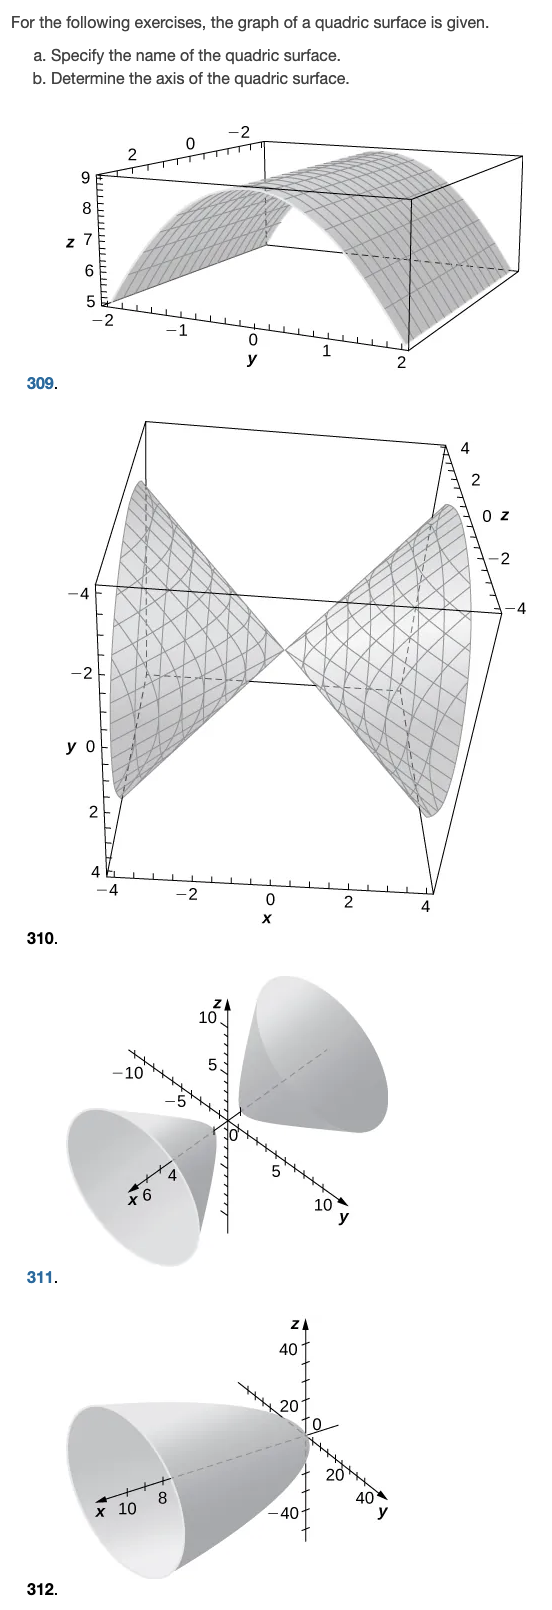
\includegraphics[scale=0.7]{assets/rec04-ex309-312.png}

\subsection{Section 2.6, Example 2.59 Identifying Equations of Quadric Surfaces}
Identify the surfaces represented by the given equations.
\begin{enumerate}[label=(\alph*)]
  \item $16x^2 + 9y^2 + 16z^2 = 144$
  \textbf{Solution}
  Observe that all the terms are squared, and all the coefficients are positive (but not equal) so this is an ellipsoid.
  % \begin{align*}
  %   \\ \\
  % \end{align*}
  \item $9x^2 - 18x + 4y^2 + 16y - 36z + 25 = 0$
  % \begin{align*}
  %   \\ \\
  % \end{align*}
  \textbf{Solution}
  We have two squared terms, and $z$ term of degree one. We could rearrange this to get $36z = 9x^2 - 18x + 4y^2 + 16y + 25$, which appears to be a elliptic paraboloid.
\end{enumerate}

\subsection{Section 2.6, Checkpoint 2.54}
Identify the surface represented by the equation $9x^2 + y^2 - z^2 + 2z - 10 = 0$.

\textbf{Solution} We have three squared terms, two positive coefficients and one negative coefficient. So this is a double cone.
% \begin{align*}
%   \\ \\
% \end{align*}

\subsection{Section 2.6, Exercise 350}
Find the equation of the quadric surface with points $P(x,y,z)$ that are equidistant from point $Q(0,2,0)$ and plane of equation $y=-2$. Identify the surface. 

\textbf{Solution} First, the distance from a point $(x, y, z)$ to the plane $y = -2$ is just $\abs{y}$. \textit{This is because the plane $y = -2$ has normal vector $\hat{j}$; projecting $\overrightarrow{PQ}$ onto $\hat{j}$ just yields the $y$ component.}

To do this, we want $\langle x, y, z \rangle$ that satisfies
\begin{align*}
  \sqrt{(x-0)^2 + (y-2)^2 + (z-0)^2} &= y - (-2) 
  \\ \sqrt{x^2 + (y-2)^2 + z^2} &= y + 2
  \\ x^2 + (y-2)^2 + z^2 &= (y+2)^2
  \\ x^2 + y^2 - 4y + 4 + z^2 &= y^2 + 4y + 4
  \\ x^2 + z^2 &= 8y
\end{align*}
This is the form of an elliptic paraboloid.

\newpage
\section{09-09-2025}
\subsection{Section 3.1, Exercise 8}
Find the limit of the following vector valued function at the indicated value of $t$.
\[\lim_{t\to 4}\left\langle \sqrt{t-3}, \dfrac{\sqrt{t} - 2}{t-4}, \tan\left(\dfrac{\pi}{t}\right)\right\rangle\]
\textbf{Solution} We can just substitute for the $x$ and $z$ components. The middle one requires more thought; direct substitution gives $\frac{0}{0}$, so we apply L'Hopital's rule.
\[\lim_{t\to 4} \dfrac{\sqrt{t}-2}{t-4} = \lim_{t\to 4} \dfrac{\frac{1}{2\sqrt{t}}}{1} = \dfrac{1}{4}\]
So the limit is 
\[\left\langle1, \dfrac{1}{4}, 1\right\rangle\]
% \begin{align*}
%   \\ \\ \\ \\
% \end{align*}

\subsection{Section 3.1, Exercise 22}
Eliminate the parameter $t$, write the equation in Cartesian coordinates, then sketch the graphs of the vector-valued functions. \textit{Hint: solve first equation for $x$ in terms of $t$ and substitute this result into the second equation}.
\[\mathbf{r}(t) = 2t \hat{i} + t^2 \hat{j} \qquad \text{let }x=2t, y=t^2\]
\begin{align*}
  \\ \\ \\ \\ \\ \\
\end{align*}

\begin{center}
  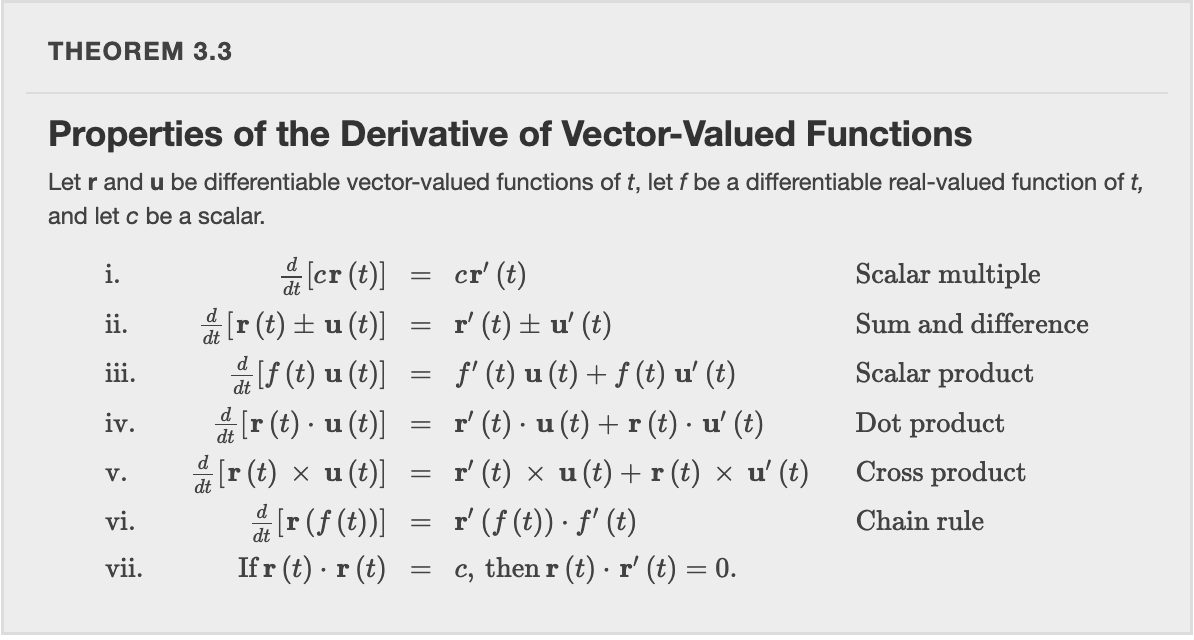
\includegraphics[scale=0.6]{assets/rec05-derivative-properties.png}
\end{center}

\newpage
\subsection{Section 3.2, Checkpoint 3.5}
Calculate the derivative of the function 
\[\mathbf{r}(t) = (t\ln t)\hat{i} + (5e^t)\hat{j} + (\cos t - \sin t)\hat{k}\]
\begin{align*}
  \\ \\ \\ \\ \\ \\
\end{align*}

\subsection{Section 3.2, Checkpoint 3.7}
Find the unit tangent vector for the vector-valued functions
\[\mathbf{r}(t) = (t^2-3)\hat{i} + (2t+1)\hat{j} + (t-2)\hat{k}\]
\begin{align*}
  \\ \\ \\ \\ \\ \\
\end{align*}

\subsection{Section 3.2, Checkpoint 3.8}
Calculate the following integral:
\[\int_{1}^{3}\left[(2t+4)\hat{i} + (3t^2 - 4t)\hat{j}\right] \ dt\]

\newpage
\section{09-11-2025}
\subsection{Section 3.3, Checkpoint 3.9}
Calculate the arc length of the parameterized curve
\[\mathbf{r}(t) = \langle 2t^2 + 1, 2t^2 - 1, t^3 \rangle, \quad 0 \le t \le 3\]
\begin{align*}
  \\ \\ \\ \\ \\ \\ \\ \\ \\ \\
\end{align*}
Extension: write the arc length parametrization by solving for $t$ in terms of $s$
\begin{align*}
  \\ \\ \\ \\
\end{align*}

\newpage
\subsection{Section 3.3, Checkpoint 3.13}
Find the equation of the osculating circle of the curve defined by the vector-valued function 
\[y = 2x^2 - 4x + 5 \text{ at } x = 1\]
\begin{align*}
  \\ \\ \\ \\ \\ \\ \\ \\ \\ \\
\end{align*}

\subsection{Section 3.3, Exercise 3.143}
Find the equation for the osculating plane at point $t = \dfrac{\pi}{4}$ on the curve 
\[\mathbf{r}(t) = \cos(2t) \hat{i} + \sin(2t)\hat{j} + t\hat{k}\]
% Checkpoint 3.9 + write the arc length parametrization by solving for t in terms of s (answer: t = sqrt (s^(2/3) - 32/9))

\newpage
\section{09-16-2025 - Midterm 1 tomorrow}
Logistics: see @35 on Piazza.
\begin{itemize}
  \item 50 mins 
  \item no electronics at all 
  \item single-page, typical 8.5x11 or A4 size paper, front and back, can typeset or handwrite
  \item write your answer in the provided answer box so we can grade faster
\end{itemize}
Points, vectors, lines, planes, quadrics. See the handout for quadrics that I gave out, and consult the wikipedia if you need help making your formula sheet.

Dot and Cross products and their meanings
\begin{itemize}
  \item how does the dot product relate to projections/components?
  \item how does the cross product relate to areas/volumes?
  \item how do dot and cross products help when calculating work and torque?
\end{itemize}

Calculus on vector-valued functions (limits, derivatives, integrals)
\begin{itemize}
  \item Remember examples from previous recitations - sometimes we had you do L'Hopital's or do questions that required knowledge of limits from 2-D calculus.
\end{itemize}

Arc length + arc length parameterization 
\begin{itemize}
  \item What is the formula?
\end{itemize}

Curvature + unit tangent, normal, binormal
\begin{itemize}
  \item Also includes osculating planes/circles 
  \item know the formulas (or write them down on your formula sheet)
\end{itemize}

motion in space 
\begin{itemize}
  \item apply what you know about projections/components to find out the ``component'' of the tangential/normal components of acceleration
  \item plus other questions regarding position, velocity, speed, acceleration.
\end{itemize}

What can I do to study?
\textbf{DO A PRACTICE TEST} and check your answers afterwards. Read up on the textbook (see @35 on Piazza for which sections to ignore) and get a good night's sleep. I will be proctoring your exam, so I'll see you all tomorrow :-)

\newpage
\section{09-18-2025 - Post Midterm 1, No Content}

\newpage
\section{09-23-2025}
\subsection{Section 4.1, Checkpoint 4.4}
Find the domain and range of the function $f(x, y) = \sqrt{36 - 9x^2 - 9y^2}$
\begin{align*}
  \\ \\ \\
\end{align*}
\subsection{Section 4.1, Checkpoint 4.5}
Find the equation of the level surface of the function 
\[g(x, y, z) = x^2 + y^2 + z^2 - 2x + 4y - 6z\]
corresponding to $c = 2$, and describe the surface, if possible.
\begin{align*}
  \\ \\ \\
\end{align*}
\subsection{Section 4.2, Exercise 60}
\[\text{Evaluate }\lim_{(x, y)\to(1, 2)}x \text{ or explain why the limit does not exist.}\] % direct evaluation
\begin{align*}
  \\
\end{align*}
\subsection{Section 4.2, Exercise 77}
\[\text{Evaluate } \lim_{(x, y)\to(0, 0)}\ln (x^2 + y^2) \text{ or explain why the limit does not exist.} \]
\textit{Does the limit exist on \textbf{any} path?}

\newpage
\subsection{Section 4.2, Exercise 81}
\[\text{Evaluate }\lim_{(x, y)\to(0, 0)} \dfrac{x^4 - 4y^4}{x + 2y^2} \text{ or explain why the limit does not exist.}\]
\textit{Do you see any algebraic manipulations?}
\begin{align*}
  \\ \\
\end{align*}

\subsection{Section 4.2, Exercise 86}
\[\text{Evaluate }\lim_{(x, y)\to(0, 0)} \dfrac{xy + y^3}{x^2 + y^2} \text{ or explain why the limit does not exist.}\]
\begin{enumerate}[label=(\alph*)]
  \item Along the $x$-axis ($y=0$)
  \begin{align*}
  \\ \\
  \end{align*}
  \item Along the $y$-axis $x = 0$
  \begin{align*}
  \\ \\
  \end{align*}
  \item Along the path $y = 2x$
  \begin{align*}
  \\ \\
  \end{align*}
\end{enumerate}

\subsection{Section 4.2, Exercise 88}
\[\text{Evaluate }\lim_{(x, y)\to(0, 0)}\dfrac{x^2y}{x^4 + y^2} \text{ or explain why the limit does not exist.}\]
\begin{enumerate}[label=(\alph*)]
  \item Along the $x$-axis ($y=0$)
  \begin{align*}
  \\ \\
  \end{align*}
  \item Along the $y$-axis $x = 0$
  \begin{align*}
  \\ \\
  \end{align*}
  \item Along the path $y = x^2$
  \begin{align*}
  \\ \\ \\
  \end{align*}
\end{enumerate}

\subsection{Section 4.2, Exercise 95}
Determine the region in which the function is continuous. Explain your answer 
\[f(x, y) = \begin{cases}
  \dfrac{x^2y}{x^2 + y^2} & \text{if } (x,y)\neq(0,0)
  \\ 0 & \text{if }(x, y) = (0, 0)
\end{cases}\]
\textit{Hint: maybe this coordinate system isn't helpful. Also remember the Squeeze Theorem?}
\begin{align*}
  \\ \\ \\ \\ \\ \\ \\ \\
\end{align*}
\textit{We do NOT expect you to use Squeeze Theorem with completely general functions}


\newpage
\section{09-25-2025}
\subsection{Section 4.3, Checkpoint 4.13}
Calculate $\dfrac{\partial f}{\partial x}$ and $\dfrac{\partial f}{\partial y}$ for the function $f(x, y) = \tan(x^3 - 3x^2 y^2 + 2y^4)$ by holding the opposite variable constant, then differentiating.
\begin{align*}
  \\ \\ \\
\end{align*}

\subsection{Section 4.3, Exercises 114-117}
Calculate the sign of the partial derivative using the graph of the surface $f$ below.
\\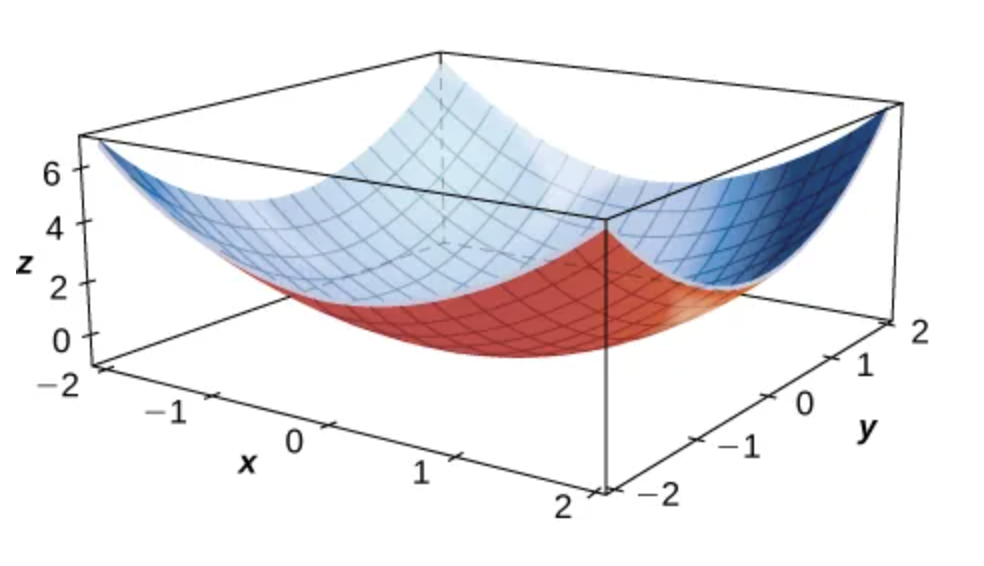
\includegraphics[scale=0.4]{assets/rec10-ex114-117.png}
\begin{enumerate}[start=114]
  \item $f_x(1, 1)$
  \item $f_x(-1, 1)$
  \item $f_y(1, 1)$
  \item $f_x(0, 0)$
\end{enumerate}
\subsection{Section 4.4, Checkpoint 4.19}
Find the equation of the tangent plane to the surface defined by the function 
\[f(x, y) = x^3 - x^2 y + y^2 - 2x + 3y - 2 \text{ at the point }(-1, 3)\]

\newpage
\subsection{Section 4.4, Checkpoint 4.22}
Find the differential $dz$ of the function 
\[f(x, y) = 4y^2 + x^2 y - 2xy\]
and use it to approximate $\Delta z$ at point $(1, -1)$. Use $\Delta x = 0.03$ and $\Delta y = -0.02$.
What is the exact value of $\Delta z$?


\newpage
\section{09-30-2025}
\subsection{Section 4.5, Checkpoint 4.23}
\subsection{Section 4.5, Exercise 253}
\subsection{Section 4.5, Example 4.30}
\subsection{Section 4.6, Example 4.31}
\subsection{Section 4.6, Example 4.32}
\subsection{Section 4.6, Checkpoint 4.30}


\newpage
\section{10-02-2025}
\subsection{Section 4.7, Checkpoint 4.35}
\subsection{Section 4.7, Checkpoint 4.36}


\newpage
\section{10-07-2025 - Midterm 2 tomorrow}
\subsection{Section 4.8, Exercise 369}
\subsection{Section 4.8, Exercise 373}
\subsection{Section 4.8, Exercise 374}
\subsection{Section 4.8, Exercise 379}
\subsection{Section 4.8, Exercise 388}


\newpage
\section{10-09-2025 - Post Midterm 2, No Content}

\newpage
\section{10-21-2025}

\newpage
\section{10-23-2025}

\newpage
\section{10-28-2025}

\newpage
\section{10-30-2025}

\newpage
\section{11-06-2025}

\newpage
\section{11-11-2025 - Midterm 3 tomorrow}

\newpage
\section{11-13-2025 - Post Midterm 3, No Content}

\newpage
\section{11-18-2025}

\newpage
\section{11-20-2025}

\newpage
\section{11-25-2025}

\newpage
\section{12-02-2025 - Final Review}

\newpage
\section{12-04-2025 - Final Review}
\end{document}